\documentclass[text07.tex]{subfiles}
\begin{document}
% \subsection*{3−1　CGIについて勉強しよう}

%
% subsection 6.4
%
\section{CGIについて勉強しよう}
% \refstepcounter{PagePtr}\label{P:CGI}
ここではCGIについて勉強しましょう。第１回で作成したwebページはいわば静的なページです。
静的なページとは、常に同じ画面を表示するページのことです。
ですが、CGI（Common Gateway Interface）を用いることによって動きのあるページ、動的なページを作成することができます。
動的なページとは表示させるたびに違う画面を表示することができるページのことです。アクセスカウンタはたまにwebページについていることがあります。

\begin{itemize}
  \item 静的ページ：いつアクセスしても内容が同じページ
  \item 動的ページ：アクセスの度に内容が変わるページ
\end{itemize}

アクセスカウンタというのは、そのwebページに今までどれぐらいの人がアクセス（接続）したのかを表示させるものです。
webページにアクセスするたびにアクセスカウンタの数は\ruby{増}{ふ}えていき、毎回同じ数字にはなりません。
これはアクセスするというアクションによってページに変化を起こしているのです。
さらにCGIを用いることによって以下の機能を作成することができます。

\bigskip

% \begin{center}
%   \label{P:slide_p28}
%   \begin{minipage}{\textwidth}
%           \begin{minipage}{0.45\textwidth}
% 	   \textbf{・アクセスカウンター}\\
% 	   \centering
%             {\upshape
%               \centering
%               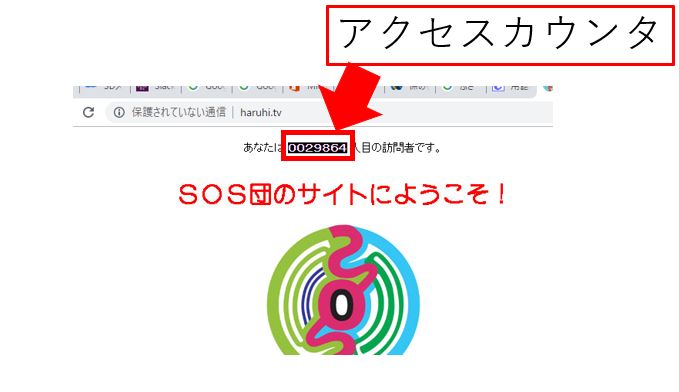
\includegraphics[width=0.8\linewidth]{../../asset/image/ome7-img046.png}}
%           \end{minipage}
%           \begin{minipage}{0.45\textwidth}
% 	   \textbf{・アンケートフォーム}\\
% 	   \centering
%             {\upshape
%               \centering
%               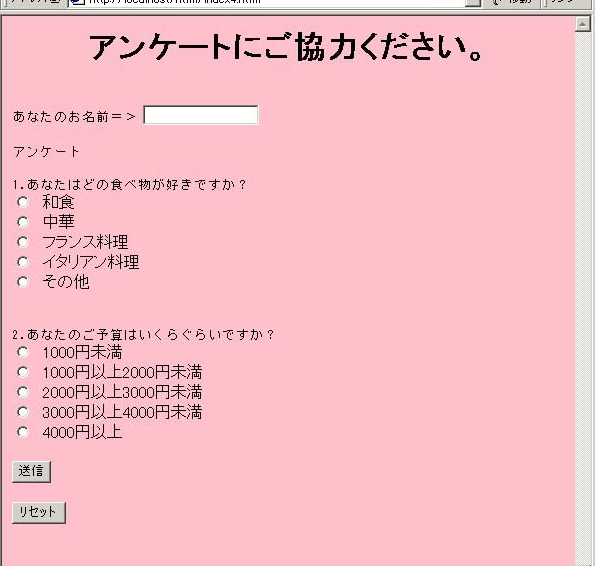
\includegraphics[width=0.8\linewidth]{../../asset/image/ome7-img047.png}}
%             \end{minipage}
%   \end{minipage}
% \end{center}
\begin{figure}[htbp]
  \centering
  \begin{minipage}{0.45\textwidth}
    \centering
    \textbf{・アクセスカウンター}\\
    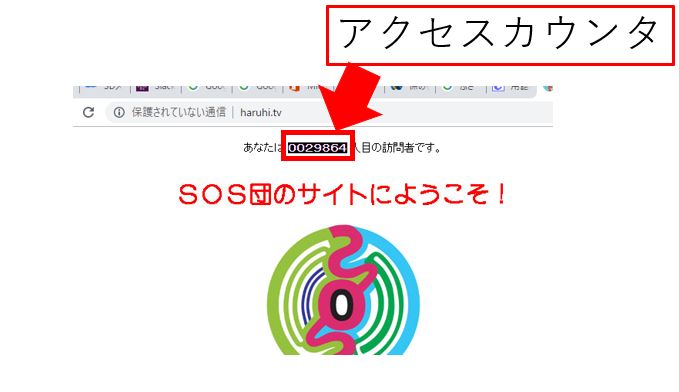
\includegraphics[width=0.8\linewidth]{../../asset/image/ome7-img046.png}
  \end{minipage}
  \hfill
  \begin{minipage}{0.45\textwidth}
    \centering
    \textbf{・アンケートフォーム}\\
    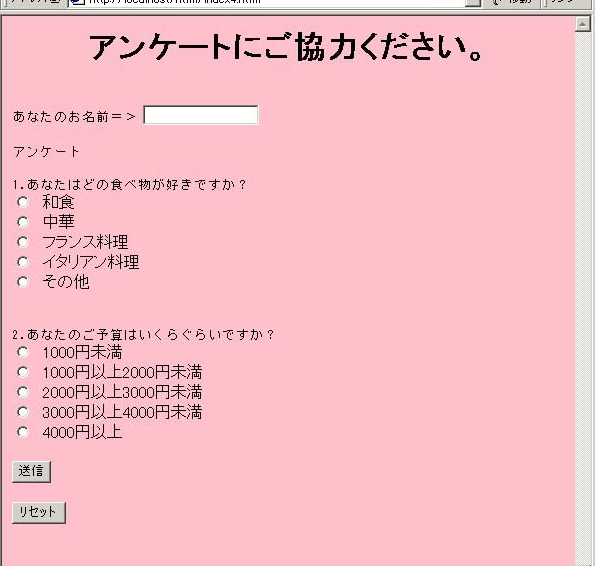
\includegraphics[width=0.8\linewidth]{../../asset/image/ome7-img047.png}
  \end{minipage}
  \label{P:slide_p28}
\end{figure}

\bigskip

{\bfseries ・\ruby{掲示板}{けいじばん}}


\begin{center}
  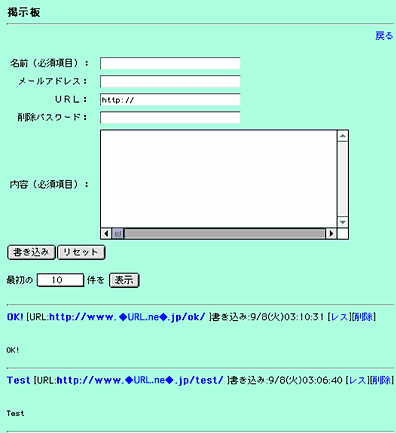
\includegraphics[width=4.431cm]{../../asset/image/ome7-img048.png}
\end{center}

みんなが作ったwebページやほかの静的なページはどのようなやり取りで表示させているか見ていきましょう。次の図を見てください。


\clearpage

\begin{center}
  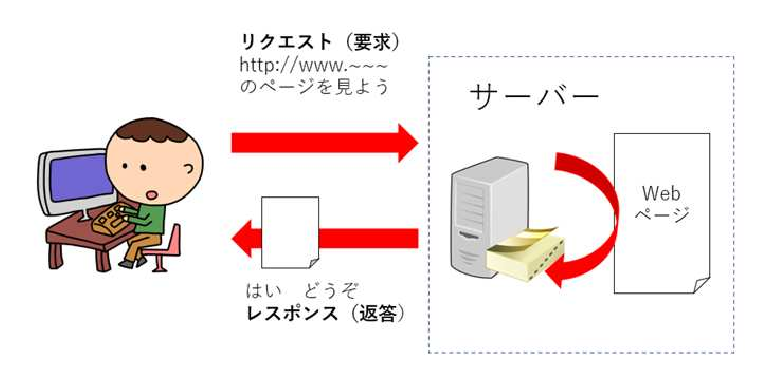
\includegraphics[width=0.75\textwidth]{../../asset/image/ome7-img049}
\end{center}

webブラウザで検索したりしてwebページを表示させることをリクエスト（要求）といい、そのリクエストを受け取ったそのwebページのあるサーバが要求したところにレスポンス（返答）を返します。
要求されたら返すのみで、webページに変化はなく同じものを見せていました。
ですが次の画像をみてください。

\begin{center}
  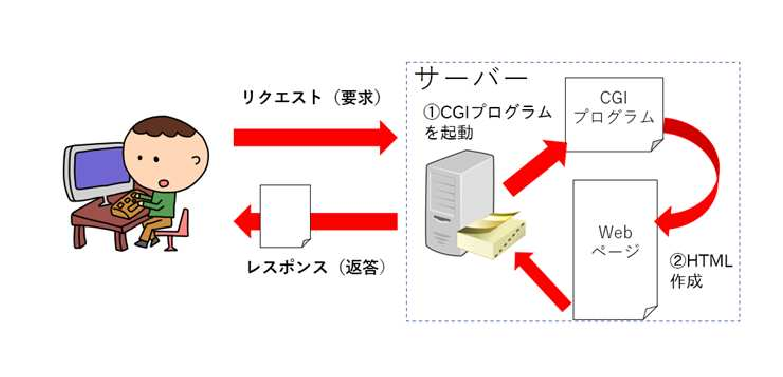
\includegraphics[width=0.75\textwidth]{../../asset/image/ome7-img050}
\end{center}


CGIを使った動的ページでは、サーバが皆さんからwebページを要求されるたびに、CGIプログラムで新しいHTMLを生成しています。
それにより、毎回違うwebページを見せることが可能なのです。
この教科書では皆さんのラズベリーパイと今までの講義で学んだことを生かしたCGIを体験していきます。

\begin{tcolorbox}[title=\useOmetoi,breakable]\label{Q:dynamicPage}
  \begin{enumerate}
    \addquiz{動的なページとはどのようなものでしょうか。}
    \addquiz{動的なページを作成する場合に用いるものは何でしょう。}
  \end{enumerate}
\end{tcolorbox}

\clearpage


% \refstepcounter{Question}\theQuestion　動的なページとはどのようなものでしょうか。また、動的なページを作成する場合に用いるものは何でしょう。\label{Q:dynamicPage}\\


% % 問題7-9　　
% % 動的なページとはどのようなものでしょうか。また、動的なページを作成する場合に用いるものは何でしょう。


% 　　

% 　　

% 　　

% 　　
% 　　
% 　　
% 　　
% 　　
% 　　


% {\bfseries 
%     \underline{答え:　　　　　　　　　　　　　　　　　　　　　　　　　　　　　　　　　　　　　　　　　　　　　}
% }

% 　　

% 　　

% 　　

% 　　
% 　　
% 　　
% 　　
% 　　
% 　　



% {\bfseries 
%     \underline{答え:　　　　　　　　　　　　　　　　　　　　　　　　　　　　　　　　　　　　　　　　　　　　　}
% }

\end{document}
